\documentclass{report}
\usepackage[utf8]{inputenc}
\usepackage{amsmath}
\usepackage{graphicx}
\usepackage{amsfonts}
\usepackage{amssymb}

\title{Eksamensnoter - Amortized Analysis}
\author{André Oskar Andersen (wpr684)}
\date{\today}

\begin{document}
\maketitle

\section*{24.1 - 1}
\textbf{Run the Bellman-Ford algorithm on the directed graph of Figure 24.4, using vertex $z$ as the source. Show the $d$ and $\pi$ values after each pass. Now, change the weight of edge $(z, x)$ to 4 and run the lagorithm again, using $s$ as the source}
\begin{center}
    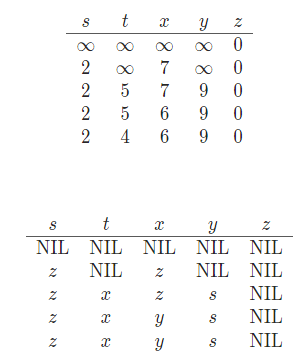
\includegraphics[width = 6 cm]{../entities/24_1_1_first.png}
    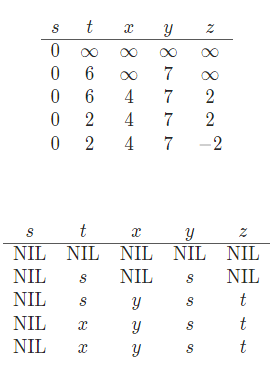
\includegraphics[width = 6 cm]{../entities/24_1_1_second.png}
\end{center}

\textbf{Prove Corollary 24.3} \\
Suppose there is a path from $s$ to $v$. Then there must be a shortest such path of length $\delta(s, v)$. It must have finite length since it contains at most $|V| - 1$ edges and each edge has finite length. By Lemma 24.2, $v.d = \delta(s, v) < \infty$ ipon termination.

\end{document}